\section{Zadanie 2}

W zadaniu nr 2 celem było wyznaczenie estymowanych faktorów na podstawie syntetycznie wygenerowanych obserwacji. Należało je wykonać za pomocą wybranego algorytmu NTF.

\subsection{Implementacja}

Na poniższym listingu został przedstawiony początkowy fragment implementacji rozwiązania zadania. Pierwszą czynnością do wykonania jest przypisanie zadanych danych do zmiennych oraz wygenerowanie faktorów $U^{(1)}$, $U^{(2)}$ i $U^{(3)}$ (odpowiednio zmienne: \textit{U1w}, \textit{U2w} i \textit{U3w}). Następnie, na podstawie tychże faktorów oraz macierzy jednostkowej \textit{I} o wymiarach \textit{JxJxJ}, generowane są trójwymiarowe, syntetyczne obserwacje \textit{Y}. W tym celu została wykorzystana funkcja \textit{ntimes}, mnożąca ze sobą kolejno po dwie podane macierze. \textit{Y} to tensor o wymiarach 10x20x30 - jest to złożenie dłuższego wymiaru każdego ze stworzonych faktorów. \\

\begin{minipage}{\linewidth}
\begin{lstlisting}[linewidth=14.5cm]
% Dane
I1 = 10;
I2 = 20;
I3 = 30;
J = 5;

% Inicjalizacja faktorow
U1w = max(0, randn(I1, J));
U2w = max(0, randn(I2, J));
U3w = max(0, randn(I3, J));

% Syntetyczne obserwacje Y 
I = zeros(J,J,J);
for i = 1 : J
	I(i,i,i) = 1;   
end

Y = ntimes(ntimes(ntimes(I, U1w, 1, 2), U2w, 1, 2), U3w, 1, 2);

%% Algorytm ALS
% Inicjalizacja faktorow
U1 = randn(I1, J);
U2 = randn(I2, J);
U3 = randn(I3, J);

% Matrycyzacja Y wzgledem poszczegolnych modow
Y1 = reshape(permute(Y,[1,2,3]),size(Y,1),size(Y,2)*size(Y,3));
Y2 = reshape(permute(Y,[2,1,3]),size(Y,2),size(Y,1)*size(Y,3));
Y3 = reshape(permute(Y,[3,1,2]),size(Y,3),size(Y,1)*size(Y,2));

% Obliczenie wersji 2-D tensora Y
Y_2d = reshape(Y,size(Y,1),size(Y,2)*size(Y,3));
\end{lstlisting}
\end{minipage}
\vspace{5mm}

Kolejnym krokiem jest dekompozycja CP z wykorzystaniem algorytmu ALS. Inicjalizowane są estymowane faktory (zmienne \textit{U1}, \textit{U2} i \textit{U3}). Algorytm wymaga matrycyzacji tensora \textit{Y} względem poszczególnych modów, co udało się uzyskać używając funkcji reshape i permute. Oznacza to, że macierze wyjściowe \textit{Y1}, \textit{Y2} i \textit{Y3} są dwuwymiarowe - pierwszy z wymiarów jest równy kolejnemu wymiarowi oryginalnego \textit{Y}, a drugi - iloczynem pozostałych wymiarów. Ostatnia czynność to obliczenie dwuwymiarowej wersji tensora \textit{Y}, potrzebnej do późniejszego wyznaczenia błędu residualnego (funkcja \textit{norm} przyjmuje jako argumenty jedynie dwuwymiarowe macierze).\\

\vspace{5mm}
\begin{minipage}{\linewidth}
\begin{lstlisting}[linewidth=14.5cm]
MaxIter = 200;
for k = 1: MaxIter

	% Update naprzemienny faktorow i normalizacja
	A1 = max(0,(kr(U3,U2))');    
	U1 = max(0, (Y1*A1')/(A1*A1'));
	U1 = U1*(diag(1./sum(U1, 1)));
	
	A2 = max(0,(kr(U3, U1))');    
	U2 = max(0, (Y2*A2')/(A2*A2'));
	U2 = U2*(diag(1./sum(U2, 1)));
	
	A3 = max(0,(kr(U2,U1))');
	U3 = max(0, (Y3*A3')/(A3*A3'));
	
	% Wyliczanie tensora Yk na dla k-tej iteracji
	% na podstawie aktualnych U1, U2 i U3
	Yk = ntimes(ntimes(ntimes(I,U1,1,2),U2,1,2),U3,1,2);
	Yk_2d = reshape(Yk,size(Yk,1),size(Yk,2)*size(Yk,3));
	
	% Blad residualny
	res(k) = norm(Y_2d - Yk_2d, 'fro')/norm(Y_2d, 'fro');
end

% Rysowanie wykresu bledu
semilogy(res)

% Jakosc estymacji
mse = immse(Y, Yk);
\end{lstlisting}
\end{minipage}
\vspace{5mm}

Na listingu widocznym powyżej przedstawiona jest główna pętla działania programu. W każdym przebiegu pętli wyznaczane są wartości faktorów \textit{U1}, \textit{U2} i \textit{U3}. Wykonywana jest także ich normalizacja. Obliczana jest także wartość \textit{Yk}, czyli wartości tensora \textit{Y} dla faktorów wyznaczonych w danej iteracji. Następnie z \textit{Yk} powstaje macierz dwuwymiarowa \textit{Yk\_2d}. Na podstawie \textit{Yk\_2d} i \textit{Y\_2d} wyliczany jest błąd residualny dla aktualnie wyznaczonej wartości \textit{Yk}.\\
Podsumowanie wyników obliczeń polega na narysowaniu wykreu błędu residualnego w kolejnych iteracjach oraz wyliczenie błędu średniokwadratowego.

\vspace{5mm}



\subsection{Wyniki}

Na wykresie \ref{rys:zad2_res} można zaobserwować zmiany wartości błędu residualnego w kolejnych iteracjach algorytmu. W omawianym przypadku stabilizuje się ona między 40 a 50 przebiegiem pętli. Dalsze iteracje nie wpływają znacząco na wynik obliczeń.

\begin{figure}[H]
	\centering
	\hspace*{-1.2in}
	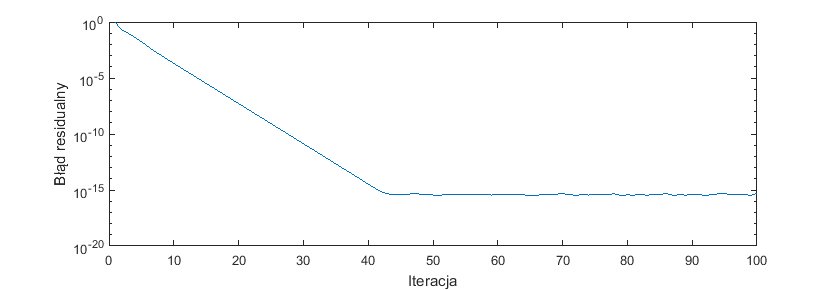
\includegraphics[scale = 0.9]{zad2_res.png}
	\caption{Unormowany błąd residualny w danej iteracji dla funkcji iteracji naprzemiennych}  
	\label{rys:zad2_res} 
\end{figure}

Powyższe obserwacje potwierdza także otrzymana z obliczeń wartość błędu średniokwadratowego. Po 50 iteracjach wynosi on $2.3831\mathrm{e}{-31}$, natomiast po 100 przebiegach pętli - $2.1673\mathrm{e}{-31}$. Wynik został więc ustabilizowany.